\documentclass[tikz,convert={outext=.svg,command=\unexpanded{pdf2svg \infile\space\outfile}},multi=false]{standalone}
\usepackage[utf8]{inputenc}

\begin{document}
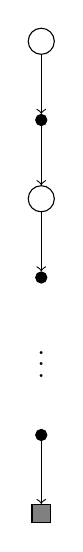
\begin{tikzpicture}
\tikzstyle{state} = [draw, circle, fill=white];
\tikzstyle{action} = [draw, circle, fill=black, inner sep=0.5mm];
\tikzstyle{finalstate} = [draw, fill=gray];
\node[state] (s) {};
\node[action] (a) at (0, -1) {};
\node[state] (s') at (0, -2) {};
\node[action] (a') at (0, -3) {};
\node[action] (a'') at (0, -5) {};
\node[finalstate] (s'') at (0, -6) {};
\node (.) at (0, -4) {$\vdots$};
\draw[->] (s) -- (a);
\draw[->] (a) -- (s');
\draw[->] (s') -- (a');
\draw[->] (a'') -- (s'');
\end{tikzpicture}
\end{document}